\documentclass{article}


%INCLUDE
\usepackage[a4paper, left=20mm, right=20mm, top=20mm, bottom=20mm]{geometry}

\usepackage{amsmath, amsthm}
\usepackage[T1,T2A]{fontenc}
\usepackage[utf8]{inputenc}
%\usepackage[russian]{babel}
\usepackage{amssymb}
\usepackage{hyperref}
\usepackage{stackengine}
\usepackage{algorithm}
\usepackage{algpseudocode}
\usepackage{lipsum}
\usepackage{authblk}
\usepackage{graphicx}
\usepackage{multicol}
\usepackage{pgfplots}
\usepackage{bm}
\usepackage{subcaption}
\usepackage{float} % for the H specifier


%KHALED BEGIN

\usepackage{natbib}
\setcitestyle{authoryear,round,citesep={;},aysep={,},yysep={;}}

\renewcommand{\bibname}{References}
\renewcommand{\bibsection}{\subsubsection*{\bibname}}
\bibliographystyle{plainnat}

\usepackage[tableposition=top]{caption}
\usepackage{amsmath,amsthm,amssymb,mathtools,graphicx,enumitem,hyphenat,float, threeparttable}
\usepackage{mathabx, hyperref}
\hypersetup{ %
    pdfborder=0 0 0,
    pdfpagemode=UseNone,
    colorlinks=true,
    linkcolor=blue,
    citecolor=blue,
    filecolor=blue,
    urlcolor=blue,
    pdfview=FitH}
%KHALED END

%THEOREMS
\makeatletter
\def\th@plain{%
  \thm@notefont{}% same as heading font
}
\makeatother

\theoremstyle{plain}
\newtheorem{lemma}{Lemma}
\newtheorem{sublemma}{Sublemma}[lemma]


\theoremstyle{plain}
\newtheorem{assumption}{Assumption}

\theoremstyle{plain}
\newtheorem{corollary}{Corollary}

\theoremstyle{remark}
\newtheorem*{remark}{Remark}

\theoremstyle{plain}
\newtheorem{theorem}{Theorem}


%COMMANDS
\newcommand{\norm}[1]{\left\|#1\right\|}
\newcommand{\inner}[2]{\langle #1, #2\rangle}
\newcommand{\summ}[3]{\sum^{ #2 }_{ #1 } #3}
\newcommand{\fsumm}[3]{\frac{1}{M}\sum^{ #2 }_{ #1 } #3}
\newcommand{\coef}[1]{\biggr[ #1 \biggr]}
\newcommand{\E}{\mathbb{E}}

\begin{document}

%TITLE
%TITLE

\title{\fontsize{12}{14}\selectfont \textbf{Enhancing the convergence estimation of Local SGD for quadratic-like functions / Local SGD converges faster for quadratic-like functions independent of the Hessian}}

\author[1]{\fontsize{11}{14} \textbf{Andrei Sadchikov}}
\author[1, 2]{\fontsize{11}{14} \textbf{Aleksandr Beznosikov}}
\author[1, 3]{\fontsize{11}{14} \textbf{Alexander Gasnikov}}
\affil[1]{MIPT}
\affil[2]{University Two}
\affil[3]{University Three}

\date{}

%BEGIN
\maketitle

%ABSTRACT
\begin{abstract}
One of the challenges of Federated learning is finding the right balance in communication frequency: too infrequent communications lead to worse convergence, while too frequent ones require significant overhead (time for data transmission and network load). 
\cite{Woodworth} proved that for the case where the objective function is quadratic, the communication frequency does not affect the upper bound on the convergence rate.
In this work, we focus on generalizing these results, providing an analysis in the case where the objective function is the sum of a quadratic function and an arbitrary remainder.
\end{abstract}

%MAIN BODY
%INTRODUCTION
\section{Introduction}
$ $\par

\subsection{General words}

In the ever-evolving landscape of machine learning, we've witnessed the emergence of enormous models like Gemini, boasting trillions of parameters that push the boundaries of computational capacity. Given the impracticality of training such models on a single device, modern machine learning has embraced Federated Learning, a concept initially introduced by \cite{McMahan}. This approach involves distributing data across multiple devices, each conducting local computations, and subsequently communicating to collectively achieve the final result.

\vspace{10pt}

However, the challenge of communication frequency remains unresolved in Federated Learning. Insufficient communication may lead to divergence, while overly frequent communication poses its own set of issues. Imagine tackling an optimization problem in a space with a dimensions around $10^9$, which occurs often in practice \citep{shahid2021communication}. Each time we compute a gradient locally, it ends up being gigabytes in size, which makes sending it over for transmission quite a challenge. Thus, striking the delicate balance in communication frequency becomes the key to success in Federated Learning.

\vspace{10pt}

The scientific community has developed sophisticated federated learning frameworks that leverage the idea of rare intermittent communications. Among the most notable are SCAFFOLD \citep{Scaffold} and FedAC \citep{FedAC}. These algorithms are widely utilized in practice, particularly when data distribution varies among computational devices \citep{Hospitals}. However, the simplest and most classical algorithm, named Local SGD (also known as FedAvg or Parallel SGD, \cite{Mangasarian}), has been proven to be as efficient as these intricate algorithms when data distribution is similar \citep{KEK LOL}. 
The core concept of Local SGD can be described as follows: each participating device conducts few steps of SGD locally and then devices communicate with each other averaging their models' weights.

\vspace{10pt}

In environments where the distribution of data remains consistent, such as when computations are distributed within a computational cluster or among processor cores within a single device, Local SGD finds extensive application. This classical algorithm remains actively utilized in modern machine learning applications such as Natural Language Processing (NLP) and computer vision. Recent studies \citep{LocalSGD_LLM, LocalSGD_CV} have underscored its efficiency and effectiveness in identical distribution situations. With its straightforward approach and strong performance, Local SGD continues to play pivotal role in diverse domains of federated learning.

\vspace{10pt}

\subsection{Problem formulation}

Now, let us formally introduce the task we are solving. Consider a scenario where \( M \) devices \( 1, 2, \ldots, m \), collectively solving optimization problem, that is finding:

\[ x_* := \arg\min_{x \in \mathbb{R}^d} F(x) \]

Here, \( F(x) \) is defined as the expected value over a distribution \( \mathcal{D} \):

\[ F(x) := \mathbb{E}_{z \sim \mathcal{D}} [F(x, z)] \]

%where \( z \) is sampled from the distribution \( \mathcal{D} \).

Our focus lies on a first-order stochastic oracle, where we have access to the stochastic estimate of \( \nabla F \) on each node. We denote this estimate as \( \nabla F(x, z) \), with \( z \) representing a sample from \( \mathcal{D} \).

This formulation captures a wide range of practical problems, such as Empirical Risk Minimization \citep{Vapnik}. In our case \( F \) denotes the empirical risk (i.e., the average of losses across some data samples) and \( z \) denotes the indices of data samples.

\vspace{10pt}

As we have already mentioned, one of the primary frameworks for addressing such problem is Local SGD. This method involves executing few consecutive SGD steps locally on each device, averaging the results, and repeating this process for $R$ rounds, resulting in a total of $T$ iterations on each device.

\begin{algorithm} \label{alg:localsgd}
    \caption{Local SGD}
    \begin{algorithmic}[1]
        \State \textbf{Input:} 
        Initial vector $x_0 = x^m_0$ for all $m \in \{1, \ldots, M\}$; 
        stepsize $\gamma \geq 0$
        \For{$t = 1, \ldots, T = R\cdot H$}
            \For{$m = 1, \ldots, M$ in parallel}
                \State Sample $z^m_t \sim \mathcal{D}$.
                \State Evaluate stochastic gradient $\mc{g}_t^m = \nabla F(x_t^m, z^m_t)$.
            \EndFor
            \If{$t+1 \mod H = 0$}
                \State $x^m_{t+1} = \frac{1}{M} \sum^M_{j = 1} (x^j_t - \gamma \mc{g}^j_t) $
            \Else
                \State $x^m_{t+1} = x_t^m - \gamma \mc{g}_t^m$ \label{eq:upd_eq}
            \EndIf
        \EndFor
    \end{algorithmic}
\end{algorithm}

\vspace{10pt}

\subsection{Related work}

In both scenarios of identical and heterogeneous settings, extensive research has been conducted across various contexts. \citep{Li} analyzed the non-convex setting under bounded gradient norms. As expected, the further we deviate from the identical and strongly convex settings, the poorer the results become. However, in this work, we will focus solely on convex and strongly convex cases.

\vspace{10pt}

\cite{Woodworth} demonstrated that in the scenario where the objective function is quadratic, the convergence rate of Local SGD remains independent of communication frequency. This observation aligns with the lower bounds established for Local SGD, indicating that for purely quadratic functions, further enhancement of convergence rate is unattainable.

\vspace{10pt}

The most promising outcomes in the identical convex case, where the function is not quadratic, were previously achieved under the assumption of Lipschitz Hessian \citep{FedAC}. This observation resonates with the findings of \cite{FedAC} and \cite{Spiridonoff}, who concluded that closer proximity to a purely quadratic case correlates with improved convergence estimates.

\vspace{10pt}

Notably, \cite{Khaled} and \cite{Woodworth} provided the best known estimate without any restrictions of the Hessian. In our study, we extend these findings, particularly in cases where the objective function $F$ exhibits proximity to a quadratic form. Importantly, our approach does not assume Hessian Lipschitzness, thus representing a generalization of previous research efforts.




\begin{table}[H]
\centering
\begin{tabular}{|p{2.5cm}|p{1.5cm}|p{1.5cm}|p{1.5cm}|p{6cm}|}
\hline
\textbf{\footnotesize Reference} & \textbf{\footnotesize Not-Lipschitz Hessian} & \textbf{\footnotesize Unbounded Gradient} &\textbf{\footnotesize Noise model} & \textbf{\footnotesize Convergence rate $\E{\norm{r_T}^2}$} \\ \hline

{\footnotesize Vanila SGD} & \greencheck & \greencheck & {\footnotesize Uniform} & 
{
$O(exp.decay + \frac{A}{B})$ 
}

\\ \hline
{\footnotesize \cite{Stich} } & \greencheck & \redcross & {\footnotesize Uniform} & 
{\footnotesize
$O(exp.decay + \frac{A}{B})$
}

\\ \hline
{\footnotesize \cite{FedAC}} & \redcross & \greencheck & {\footnotesize Uniform} & 
{\footnotesize
$O(exp.decay + \frac{A}{B})$ 
}

\\ \hline
{\footnotesize \cite{Spiridonoff}} & \redcross & \greencheck & {\footnotesize Uniform with strong growth} & 
{\footnotesize
$O(exp.decay + \frac{A}{B})$ 
}

\\ \hline
{\footnotesize \cite{Khaled}} & \greencheck & \redcross & {\footnotesize Uniform} & 
{\footnotesize
$O(\frac{\norm{r_0}^2}{T^2} + \frac{\sigma^2}{\mu^2 MT} + \frac{\kappa \sigma^2}{\mu^2 TR})$ 
}

\\ \hline
{\footnotesize \textbf{This work}} & \greencheck & \greencheck & {\footnotesize Uniform with strong growth} & 
{\footnotesize
$O(exp.decay + \frac{\sigma^2}{\mu^2 MT} + \frac{\varepsilon  \kappa \sigma^2}{\mu^2 TR})$ 
}

\\ \hline

\end{tabular}
\caption{Comparison of results for general convex case}
\label{tab:results}
\end{table}


As evident from this table, our work achieves a clear improvement in the estimates obtained by \cite{Khaled}.

% The rest of this paper is organized as follows. In the following section we outline the related
% literature and compare existing results. In subsection~\ref{subsec:settings} we define the main problem and state our assumptions.
% We present our theoretical findings in subsection~\ref{subsec:contributions}  followed by numerical experiments in section~\ref{sec:experiments} and
% proofs in section~\ref{sec:proofs}.


%SETTINGS AND CONTRIBUTIONS
\section{Settings and Contributions} 
\subsection{Settings} \label{subsec:settings}

%Convexity and nabla-Lipschitzness
\begin{assumption} \label{ass:ass_1}
    Assume that $F$ is $\mu$-strongly convex and $L$-smooth. That is, $\forall x, y \in \mathbb{R}^d$,
    \[
    \frac{\mu}{2} \norm{x - y}^2 \leq F(y) - F(x) - \inner{\nabla F(x)}{y-x} \leq \frac{L}{2} \norm {x-y}^2
    \]
\end{assumption}

\begin{corollary} \label{cor:nesterov}
Under assumption~\ref{ass:ass_1}
    \[
    \frac{1}{2L} \norm{\nabla F(x) - \nabla F(y)} \leq F(y) - F(x) - \inner{\nabla F(x)}{y-x}
    \]
\end{corollary}
\proof{
    This is Theorem 2.1.5 in \cite{Nesterov}
}

%Bounded stochastic gradient variance
\begin{assumption} \label{ass:ass_2}
    Assume that for stochastic gradient variance is bounded, i.e. exists such $\sigma$ that:
    \[\E_{z \sim \mathcal{D}} \norm {\nabla F(x, z) - \nabla F(x)}^2 \leq \sigma^2
    + \rho \norm{\nabla F(x)}^2 \]
\end{assumption}

%F=Q+R decomposition
\begin{statement} \label{st:st_1}
    Objective function can be decomposed as $F = Q + R$, where $Q$ is a quadratic function that is $\mu_Q$-convex and $L_Q$-smooth, and $R$ is $\mu_R$-convex and $L_R$-smooth. Than we denote parameter
    \(\varepsilon := \frac{L_R}{L}\)
    which gives us an idea of how far $F$ is from a quadratic function.
\end{statement}

Note that such decomposition always takes place beacuse we can take $Q = 0$ and $R = F$.


In prospect of statement ~\ref{st:st_1}, following takes place:
\begin{corollary} \label{cor:linearity}
    $\nabla Q$ is a linear function
\end{corollary}

\begin{corollary}
    \(\varepsilon \leq 1\)
\end{corollary}

\begin{corollary} \label{cor:mu}
    \(\mu_Q + \mu_R \leq \mu\)
\end{corollary}
\subsection{Contributions} \label{subsec:contributions}

In this work, we mainly focus on the improvement in the last term of both convergence rates provided by Khaled et al. in prospect of statement~\ref{st:st_1}.

%THEOREM 1
\begin{theorem} \label{th:th_1}
    Under assumptions~\ref{ass:ass_1} and~\ref{ass:ass_2}, decomposing $F$ as announced in~\ref{st:st_1} and considering $\mu > 0$ and $\gamma \leq \frac{1}{6 L}$ gives:
    \begin{align}
        \E \norm{\bar{x}_T - x_*}^2
        \leq
        (1 - \gamma \mu)^T \norm{x_0 - x_*}^2 
        + \frac{\gamma \sigma^2}{\mu M} 
        + \frac{2 \varepsilon \gamma^2 \sigma^2 L (H-1)}{\mu}
    \end{align}
\end{theorem}

\begin{corollary} \label{}
    As it was previously shown in \cite{Woodworth}, an important special case is is achieved when epsilon is equal to zero. Than from the Theorem~\ref{th:th_1} it follows that:
    \begin{align}
        \E[\norm{\bar{x}_T - x_*}^2]
        \leq
        (1 - \gamma \mu)^T \norm{x_0 - x_*}^2 
        + \frac{\gamma \sigma^2}{\mu M}
    \end{align}
\end{corollary}

Thus, if $F$ is a quadratic function, the upper bound on the rate of convergence is independent of the communication frequency.

\begin{corollary} \label{}
    Considering $\gamma$ as a function of $t$ and choosing $\gamma_t$ as in Theorem 2 from \cite{Woodworth}, we obtain:
    \begin{align}
        \E[F(\bar{x}_t) - F(x_*)]
        \leq
        c \cdot \left(
        \text{exp} \left(-\frac{\mu T}{4 L}\right) +
        \frac{\sigma^2}{\mu MT} + \frac{\varepsilon \sigma^2}{\mu^2 TR}
        \right)
    \end{align}
    Where $c \in \mathbb{R}$ is some universal constant.
\end{corollary}



%THEOREM 2
\begin{theorem} \label{th:th_2}
    Under assumptions~\ref{ass:ass_1} and~\ref{ass:ass_2}, decomposing $F$ as announced in~\ref{st:st_1} and considering $\mu = 0$ and $\gamma \leq \frac{1}{6 L}$ we have:
    \begin{align}
        \E[F(\hat{x}_T)] - F(x_*) \leq
        \frac{2}{\gamma T} + \frac{2 \gamma \sigma^2}{M} + 12 \varepsilon \gamma^2 L \sigma^2 (H-1)
    \end{align}
    Where $\hat{x}_T = \frac{1}{T} \summ{t=1}{T} \bar{x}_t$
\end{theorem}

\begin{corollary} \label{}
    Choosing $\gamma = \frac{\sqrt{M}}{6 L\sqrt{T}}$ and assuming $M \leq T$ as in \cite{Khaled} yields:
    \begin{align}
        \E[F(\hat{x}_T)] - F(x_*)
        \leq
          \frac{12 \norm{x_0-x_*}^2}{\sqrt{MT}} + \frac{\sigma^2}{3 L\sqrt{MT}} + \frac{
          \varepsilon \sigma^2 M}{3LR}
    \end{align}
\end{corollary}


%DISCUSSION
\section{Discussion}
Things get more interesting in perspective of expressing $\E[\norm{\bar{x}_{t+1} - x_*}^2]$ through $\E[\norm{\bar{x}_{t} - x_*}^2]$ instead of solving recurrent relation and analyzing $\E[\norm{\bar{x}_T - x_*}^2]$. 

%We'll go deeper into the strongly convex case because it's more intuitive.

As can be observed from~\ref{lem:main}:
\begin{align}
     \E \norm{\bar{x}_{t+1}-x_*}^2
    &\leq
    (1 - \gamma \mu) \E \norm{\bar{x}_t - x_*}^2 
    + \frac{\gamma^2 \sigma^2}{M}
    + 10 \varepsilon \gamma L (H-1) \gamma^2 \sigma^2 \label{eq:recurrent}
\end{align}

Considering $\varepsilon$ as a function of $x$, we can say that for the functions with Lipschitz Hessian we know that the decay rate of $\varepsilon$ is fast. Following graphs illustrate decay rate of $\varepsilon$ for some functions:

\begin{figure}[H] \label{graph:eps_graphs}
\centering
\begin{subfigure}{0.3\textwidth}
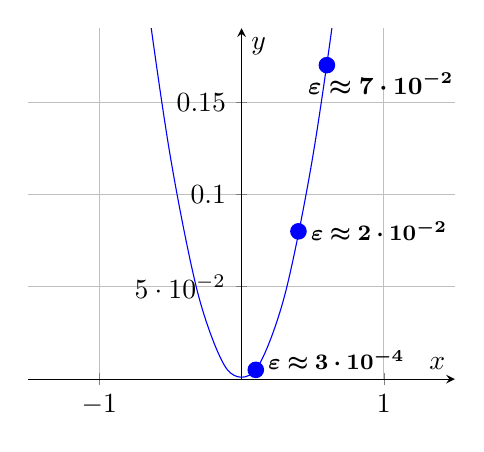
\begin{tikzpicture}
\begin{axis}[
    width=7cm,
    xlabel={$x$},
    ylabel={$y$},
    xmin=-1.5, xmax=1.5,
    ymin=0, ymax=0.19, % Adjust y-axis limits
    axis lines=center,
    grid=both,
    domain=-10:10,
    samples=100,
    % restrict y to domain=-2.5:2.5 % Restrict y-axis domain
]

\addplot[blue, smooth] {ln(cosh(x))};

\coordinate (A1) at (axis cs:0.6,0.17);
\coordinate (B1) at (axis cs:0.4,0.16);

\fill[blue, thick] (A1) circle (3pt);
\node[right] at (B1) {\small $\bm{\varepsilon \approx 7 \cdot 10^{-2}}$};

%\draw[dashed] (A1) -- (B1);
 %----------------------------------------%
\coordinate (A2) at (axis cs:0.4,0.08);
\coordinate (B2) at (axis cs:0.42,0.08);

\fill[blue, thick] (A2) circle (3pt);
\node[right] at (B2) {\footnotesize $\bm{\varepsilon \approx 2 \cdot 10^{-2}}$};

%\draw[dashed] (A2) -- (B2);
 %----------------------------------------%
% \coordinate (A3) at (axis cs:0.2,0.02);
% \coordinate (B3) at (axis cs:0.35,0.03);

% \fill[blue, thick] (A3) circle (3pt);
% \node[right] at (B3) {\footnotesize $\bm{\varepsilon \approx 2 \cdot 10^{-3}}$};

% \draw[dashed] (A3) -- (B3);
%----------------------------------------%
\coordinate (A4) at (axis cs:0.1,0.005);
\coordinate (B4) at (axis cs:0.12,0.01);

\fill[blue, thick] (A4) circle (3pt);
\node[right] at (B4) {\footnotesize $\bm{\varepsilon \approx 3 \cdot 10^{-4}}$};

%\draw[dashed] (A4) -- (B4);

\end{axis}
\end{tikzpicture}
\caption{LogCoshLoss: $y = \ln(\cosh(x))$ }
\end{subfigure}
\hfill
\begin{subfigure}{0.3\textwidth}
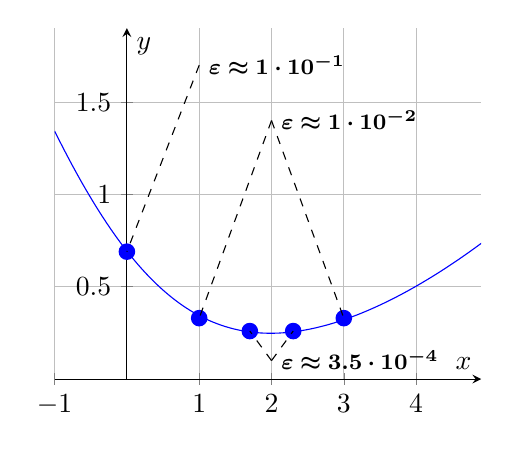
\begin{tikzpicture}
\begin{axis}[
    width=7cm,
    xlabel={$x$},
    ylabel={$y$},
    xmin=-1, xmax=4.9,
    ymin=-0, ymax=1.9,
    axis lines=center,
    grid=both,
    samples=100,
]
\addplot[blue, domain=-1:5] {-ln(1/(1 + exp(-x))) + x^2/33};

\coordinate (A1) at (axis cs:1, 0.33);
\coordinate (B1) at (axis cs:2, 1.4);
\coordinate (C1) at (axis cs:3,0.33);

\fill[blue, thick] (A1) circle (3pt);
\fill[blue, thick] (C1) circle (3pt);
\node[right] at (B1) {\footnotesize $\bm{\varepsilon \approx 1 \cdot 10^{-2}}$};

\draw[dashed] (B1) -- (A1);
\draw[dashed] (B1) -- (C1);
 %----------------------------------------%
\coordinate (A2) at (axis cs:1.7, 0.26);
\coordinate (B2) at (axis cs:2, 0.1);
\coordinate (C2) at (axis cs:2.3,  0.26);

\fill[blue, thick] (A2) circle (3pt);
\fill[blue, thick] (C2) circle (3pt);
\node[right] at (B2) {\footnotesize $ \bm{\varepsilon \approx 3.5 \cdot 10^{-4}}$};

\draw[dashed] (B2) -- (A2);
\draw[dashed] (B2) -- (C2);
 %----------------------------------------%
 \coordinate (A2) at (axis cs:0, 0.69);
\coordinate (B2) at (axis cs:1, 1.7);

\fill[blue, thick] (A2) circle (3pt);
\node[right] at (B2) {\footnotesize $\bm{\varepsilon \approx 1 \cdot 10^{-1}}$};

\draw[dashed] (B2) -- (A2);
 %----------------------------------------%
\end{axis}
\end{tikzpicture}
\caption{LogLoss with $l_2$ reg.  ~\eqref{eq:logloss}}
\end{subfigure}
\hfill
\begin{subfigure}{0.3\textwidth}
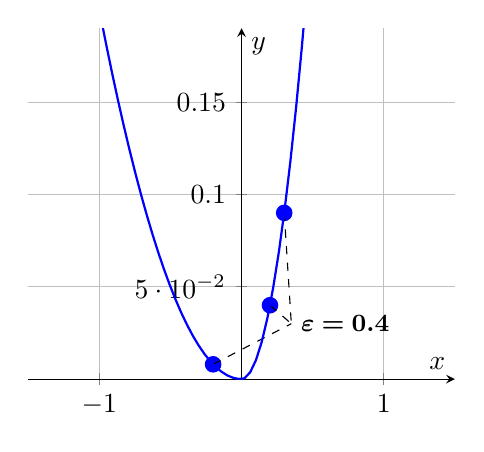
\begin{tikzpicture}[
  declare function={
    func(\x)= (\x < 0) * (x*x/5)   +
              (\x >= 0) * (x*x)
   ;
  }
]
\begin{axis}[
    width=7cm,
    xlabel={$x$},
    ylabel={$y$},
    xmin=-1.5, xmax=1.5,
    ymin=0, ymax=0.19, % Adjust y-axis limits
    axis lines=center,
    grid=both,
    domain=-2:2,
    samples=100,
    % restrict y to domain=-2.5:2.5 % Restrict y-axis domain
]

\coordinate (A1) at (axis cs:-0.2,0.008);
\coordinate (A2) at (axis cs:0.2,0.04);
\coordinate (A3) at (axis cs:0.3,0.09);

\coordinate (B1) at (axis cs:0.35,0.03);

\fill[blue, thick] (A1) circle (3pt);
\fill[blue, thick] (A2) circle (3pt);
\fill[blue, thick] (A3) circle (3pt);


\node[right] at (B1) {\small $\bm{\varepsilon = 0.4}$};

\draw[dashed] (A1) -- (B1);
\draw[dashed] (A2) -- (B1);
\draw[dashed] (A3) -- (B1);

\addplot [blue,thick] {func(x)};
\end{axis}
\end{tikzpicture}
\caption{Piecewise quadratic func. $\mathcal{F} $ ~\eqref{eq:piecewise}}
\end{subfigure}


\caption{Decay of $\varepsilon$ when getting closer to minima}
\end{figure}
\\

In point (b) by LogLoss we mean 
\begin{equation} \label{eq:logloss}
    y = -\ln\left(\frac{1}{1 + e^{-x}} \right) + 0.03 {x^2}
\end{equation}

And in point (c) we analyze well-known function that yields lower bound estimates for Local SGD \citep{LowerBound}.
\begin{equation} \label{eq:piecewise}
    \mathcal{F}(x) = \begin{cases} 
      x^2 / 5 & \text{if } x < 0 \\
      x^2 & \text{if } x \geq 0 \\
   \end{cases}
\end{equation}

Here we can notice that for functions (a) and (b) $\varepsilon$ decreases rapidly (because they satisfy Lipschitz Hessian assumption), and for function (c) it remains constant. This may be considered as some additional insight into why 
$\mathcal{F}$ yields lower bound for Local SGD.

From this example we can observe that equation~\ref{eq:recurrent} provides valuable insights into convergence rate for different types of functions. However, abandoning the assumption of a Lipschitz Hessian means that we cannot estimate the decay rate of epsilon. Therefore conducting a meaningful asymptotic analysis while maintaining generality seems impossible.

Thus our aim is to present our findings within a broader scope, elucidating the physical interpretation of the convergence rate.


%REFERENCES
\bibliographystyle{plain}
\bibliography{bibliography.bib}

%SUPPLEMENTARY MATERIAL
%CONTENTS
\tableofcontents
\newpage

%PROOFS
\section{Proofs} \label{sec:proofs}

\subsection{Notation}
$ $\par
To begin with, let us introduce useful contractions. 
By the capital Latin letters \( F, \ Q, \ R \) we will denote functions. 
Corresponding stochastic gradients will be represented by the bold Gothic lowercase Latin letters \( \mc{g}, \ \mc{q}, \ \mc{r} \), and the straight lowercase Latin letters \( g, \ q, \ r \) will denote the expectations of the gradients.

A bar above the letter (i.e., \( \bar{g} \)) will indicate that we take the average of this value among all devices.


\renewcommand{\arraystretch}{2.5} % Increase the height of each row by 50%
\begin{table}[htbp]
\centering
\begin{tabular}{|c|p{12cm}|}
\hline
\textbf{Symbol} & \textbf{Meaning} \\
\hline

$M$ & Number of devices participating in the algorithm \\

$H$ & Communication frequency - devices communicate and average their weights every $H$ iterations \\

\( x^m_t \) & Local weight on the device $m$ at time $t$ \\

\(\bar{x}_t\) & \( \fsumm{m=1}{M} x^m_t \) - average of the weights among all devices at time $t$ \\



\( \nabla F(x) \) & \( \E[\nabla F(x, z)] \) - expectation of a stochastic gradient \\

\( \bar{F}_t, \ \bar{Q}_t, \ \bar{R}_t \) & \( \fsumm{m=1}{M} F(x^m_t),\ \fsumm{m=1}{M} Q(x^m_t),\ \fsumm{m=1}{M} R(x^m_t) \) respectively \\


\( \mc{g}^m_t, \ \mc{q}^m_t, \ \mc{r}^m_t \) & \( \nabla F(x^m_t, z^m_t),\ \nabla Q(x^m_t, z^m_t),\ \nabla R(x^m_t, z^m_t) \) - corresponding stochastic gradient at time t on device $m$ \\

\( \bar{\mc{g}}_t, \ \bar{\mc{q}}_t, \ \bar{\mc{r}}_t \) & \( \fsumm{m=1}{M} \mc{g}^m_t,\ \fsumm{m=1}{M} \mc{q}^m_t,\ \fsumm{m=1}{M} \mc{r}^m_t \) - average of stochastic gradients at time $t$ \\

\( g^m_t, \ q^m_t, \ r^m_t \) & \( \nabla F(x^m_t),\ \nabla Q(x^m_t),\ \nabla R(x^m_t) \) - expected value of stochastic gradients at time t on device $m$ (namely, 
\( \E[\mc{g}^m_t], \ \E[\mc{q}^m_t], \ \E[\mc{r}^m_t] \)) \\

\( \bar{{g}}_t, \ \bar{{q}}_t, \ \bar{{r}}_t \) & \( \fsumm{m=1}{M} {g}^m_t,\ \fsumm{m=1}{M} {q}^m_t,\ \fsumm{m=1}{M} {r}^m_t \) - average of expected values of gradients at time $t$ \\

\( r_*, q_*, R_*, Q_* \) & \( \nabla R(x_*), \nabla Q(x_*), R(x_*), Q(x_*) \) - values at the optimum \\


\( V_t \) & \( \fsumm{m=1}{M} \norm{x^m_t-\bar{x}_t}^2 \) - mean deviation of $x^m_t$ from $\bar{x}_t$\\

\( D,\ \norm{r_t} \) & \( \norm{\bar{x_t} - x_*} \) - distance to the optimum at time $t$ \\

\( \kappa \) & \( \frac{L}{\lambda} \) - condition number \\

\hline

\end{tabular}
\caption{Notation summary}
\label{tab:notation}
\end{table}

\subsection{Technical lemmas}

Before demonstrating the claimed facts, let's first establish some technical results.
In this section we will follow the path of proving Lemma 3.1 from \cite{Stich}.

\begin{lemma} \label{lem:lem_1}
    \begin{align*}
        \norm{\bar{x}_t - x_* - \gamma_{t} \bar{g}_t}^2
        &= \norm{\bar{x}_t - x_*}^2 
        + \gamma_{t}^2 \norm{\bar{q}_t 
        + \bar{r}_t - q_* - r_*}^2 
        - 2 \gamma_{t} \inner{\bar{x}_t - x_*}{\bar{q}_t}
        - 2 \gamma_{t} \inner{\bar{x}_t - x_*}{\bar{r}_t} 
    \end{align*}
\begin{proof}
    \begin{align*}
        \norm{\bar{x}_t - x_* - \gamma_{t} \bar{g}_t}^2
        &= 
        \norm{\bar{x}_t - x_*}^2 
        + \gamma_{t}^2 \norm{\bar{g}_t}^2 
        - 2 \gamma_{t} \inner{\bar{x}_t - x_*}{\bar{g}_t} \\
        &= 
        \norm{\bar{x}_t - x_*}^2 
        + \gamma_{t}^2 \norm{\bar{g}_t}^2 
        - \frac{2\gamma_{t}}{M} \summ {m=1}{M}{ \inner{\bar{x}_t - x_*}{\nabla F(x^m_t)} } \\
        &= 
        \norm{\bar{x}_t - x_*}^2 
        + \gamma_{t}^2 \norm{\fsumm {m=1}{M}{\nabla F(x^m_t)}}^2 
        - \frac{2\gamma_{t}}{M} \summ {m=1}{M}{ \inner{\bar{x}_t - x_*}{\nabla F(x^m_t)} } \\
        &= 
            \notag
        \norm{\bar{x}_t - x_*}^2 
        + \gamma_{t}^2 \norm{\fsumm {m=1}{M}{\nabla F(x^m_t)} - \nabla F(x_*)}^2 
        - \frac{2\gamma_{t}}{M} \summ {m=1}{M}{ \inner{\bar{x}_t - x_*}{\nabla F(x^m_t)} } \\
        &= 
            \notag
        \norm{\bar{x}_t - x_*}^2 
        + \gamma_{t}^2 \norm{\fsumm {m=1}{M}{\nabla Q(x^m_t) + \nabla R(x^m_t) - \nabla Q(x_*) - \nabla R(x_*)}}^2  \\
        &- \frac{2\gamma_{t}}{M} \summ {m=1}{M}{ \inner{\bar{x}_t - x_*}{\nabla Q(x^m_t)} }
        - \frac{2\gamma_{t}}{M} \summ {m=1}{M}{ \inner{\bar{x}_t - x_*}{\nabla R(x^m_t)} }  \\
        &= 
        \norm{\bar{x}_t - x_*}^2 
        + \gamma_{t}^2 \norm{\bar{q}_t 
        + \bar{r}_t - q_* - r_*}^2  
        - \frac{2\gamma_{t}}{M} \summ {m=1}{M}{ \inner{\bar{x}_t - x_*}{q^m_t} }
        - \frac{2\gamma_{t}}{M} \summ {m=1}{M} { \inner{\bar{x}_t - x_*}{r^m_t} } \\
        &= 
        \norm{\bar{x}_t - x_*}^2 
        + \gamma_{t}^2 \norm{\bar{q}_t 
        + \bar{r}_t - q_* - r_*}^2 
        - 2 \gamma_{t} \inner{\bar{x}_t - x_*}{\bar{q}_t}
        - 2 \gamma_{t} \inner{\bar{x}_t - x_*}{\bar{r}_t} 
    \end{align*}
\end{proof}
\end{lemma}

\begin{lemma} \label{lem:g_t}
    Bounding the gradient norm
    \[  \norm{\bar{q}_t + \bar{r}_t - q_* - r_*}^2 \\
        \leq
        2 L_Q(1 + \zeta)  (Q(\bar{x}_t) - Q_* - \inner {q_*}{\bar{x}_t - x_*})
        + 2 L_R(1 + \frac{1}{\zeta})  (\bar{R}_t - R_* - \inner {r_*}{\bar{x}_t - x_*})
    \]
\end{lemma}
\begin{proof}
$ $\par
    By the generalized Cauchy inequality:
    \begin{align}
        &\norm{\bar{q}_t + \bar{r}_t - q_* - r_*}^2
        = \norm{\bar{q}_t - q_*}^2 
        + \norm{\bar{r}_t - r_*}^2
        + 2\inner {\bar{q}_t - q_*} {\bar{r}_t - r_*} \label{eq:St_1_1} \\
        &\leq \norm{\bar{q}_t - q_*}^2 
        + \norm{\bar{r}_t - r_*}^2 
        + \zeta \norm{\bar{q}_t - q_*}^2 
        + \frac{1}{\zeta} \norm{\bar{r}_t - r_*}^2 \label{eq:St_1_2} \\
        &= (1 + \zeta)\norm{\bar{q}_t - q_*}^2 + (1 + \frac{1}{\zeta})\norm{\bar{r}_t - r_*}^2  \label{eq:St_1_1}
    \end{align}
    
    By the $L$ - smoothness (corollary~\ref{cor:nesterov}):
    \begin{align}
        (1 + \zeta)\norm{\bar{q}_t - q_*}^2 &+ (1 + \frac{1}{\zeta})\norm{\bar{r}_t - r_*}^2 \\
        &\leq 2 L_Q(1 + \zeta)  (Q(\bar{x}_t) - Q_* - \inner {q_*}{\bar{x}_t - x_*})
        + 2(1 + \frac{1}{\zeta}) L_R (\bar{R}_t - R_* - \inner {r_*}{\bar{x}_t - x_*}) \label{eq:St_1_2}
    \end{align}
    
    Combining together \eqref{eq:St_1_1} and \eqref{eq:St_1_2}, we obtain:
    \begin{align}
        \norm{\bar{q}_t + \bar{r}_t - q_* - r_*}^2 
        \leq 2 L_Q(1 + \zeta)  (Q(\bar{x}_t) - Q_* - \inner {q_*}{\bar{x}_t - x_*})
        + 2 L_R(1 + \frac{1}{\zeta})  (\bar{R}_t - R_* - \inner {r_*}{\bar{x}_t - x_*}) \label{eq:St_1}
    \end{align}
\end{proof}


\begin{lemma} \label{lem:inner_1}
    \begin{align}
        -2 \inner{\bar{x}_t - x_*}{\bar{q}_t} &\leq 2 Q_* - 2 Q(\bar{x}_t) - \mu_Q \norm{\bar{x}_t - x_*}^2 \label{eq:St_2}
    \end{align}
\end{lemma}
\begin{proof}
    By $\mu_Q$ - convexity:
    \begin{align}
        -2 \inner{\bar{x}_t - x_*}{\bar{q}_t} &= 2 \inner{x_* - \bar{x}_t} {\bar{q}_t} \\
        &\leq 2 Q_* - 2 Q(\bar{x}_t) - \mu_Q \norm{\bar{x}_t - x_*}^2
    \end{align}
\end{proof}

\begin{lemma} \label{lem:inner_2}
\begin{align}
    \begin{split}
    - 2 \inner{\bar{x}_t - x_*}{\bar{r}_t} 
    &\leq 
    (\bar{R}_t - R_*)(\frac{1}{p} - 2) + 2 p L_R V_t - \mu_R \norm{x_* - \bar{x}_t}^2 
     - \frac{1}{p}\inner{r_*}{\bar{x}_t - x_*}
    \end{split}
\end{align}
\end{lemma}
\begin{proof}
    \begin{align}
        - 2 \inner{\bar{x}_t - x_*}{\bar{r}_t} &= 2 \inner{x_* - \bar{x}_t} {\bar{r}_t} \\
        &= \frac{2}{M} \summ{m=1}{M}{ \inner{x_* - \bar{x}_t}{r^m_t} } 
        = \frac{2}{M} \summ{m=1}{M}{\inner{x_* - x^m_t + x^m_t - \bar{x}_t}{r^m_t}} \\
        &= \frac{2}{M} \summ{m=1}{M}{\inner{x_* - x^m_t}{r^m_t}} 
        + \frac{2}{M} \summ{m=1}{M}{\inner{x^m_t - \bar{x}_t}{r^m_t}} \label{eq:St_3_0}
    \end{align}
    
    First part, by $\mu_R$ - convexity and Jensen's inequality:
    \begin{align}
        &\frac{2}{M} \summ{m=1}{M}{\inner{x_* - x^m_t}{r^m_t}} 
        \leq \frac{1}{M} \summ{m=1}{M}{2 R_* - 2 R(x^m_t) - \mu_R \norm{x_* - x^m_t}^2} \\
        &\leq \frac{1}{M} \summ{m=1}{M}{2 R_* - 2 R(x^m_t) - \mu_R \norm{x_* - \bar{x}_t}^2} 
        = 2 R_* - 2 \bar{R}_t - \mu_R \norm{x_* - \bar{x}_t}^2 \label{eq:St_3_1}
    \end{align}
    
    Second part, by the generalized Cauchy inequality:
    \begin{align}
        &\frac{2}{M} \summ{m=1}{M}{\inner{x^m_t - \bar{x}_t}{r^m_t}}
        = \frac{2}{M} \summ{m=1}{M}{\inner{x^m_t - \bar{x}_t}{r^m_t - r_*}} 
        + \frac{2}{M} \summ{m=1}{M}{\inner{x^m_t - \bar{x}_t}{r_*}} \\
        &= 
        \frac{2}{M} \summ{m=1}{M}{\inner{x^m_t - \bar{x}_t}{r^m_t - r_*}} 
        \leq \frac{2}{M} \summ{m=1}{M}{p L_R \norm{x^m_t - \bar{x}_t}^2 }
        + \frac{1}{M} \summ{m=1}{M}{\frac{1}{2 p L_R} \norm{r^m_t-r_*}^2 } \\
        &= 
        2 p L_R V_t 
        + \frac{1}{M} \summ{m=1}{M}{\frac{1}{2 p L_R} \norm{r^m_t-r_*}^2 } \label{eq:St_3_2_1}
    \end{align}
    
    By the corollary~\ref{cor:nesterov}:
    \begin{align}
        \norm{r^m_t-r_*}^2 \leq 2L_R (R(x^m_t) - R_* - \inner {r_*}{x^m_t - x_*}) \label{eq:St_3_2_2}
    \end{align}
    
    Substituting \eqref{eq:St_3_2_2} into \eqref{eq:St_3_2_1}, we complete the second part:
    \begin{align}
        &\frac{2}{M} \summ{m=1}{M}{\inner{x^m_t - \bar{x}_t}{r^m_t}}
        \leq 2 p L_R V_t 
        + \frac{1}{pM} \summ{m=1}{M}{R(x^m_t) - R_* - \inner {r_*}{x^m_t - x_*} } \\
        &\leq 2 p L_R V_t 
        + \frac{1}{p} (\bar{R}_t - R_* - \inner {r_*}{\bar{x}_t - x_*}) \label{eq:St_3_2}
    \end{align}
    
    Combining together \eqref{eq:St_3_0}, \eqref{eq:St_3_1}, \eqref{eq:St_3_2}, we gain:
    \begin{align}
         - 2 \inner{\bar{x}_t - x_*}{\bar{r}_t} &\leq
         2 R_* - 2 \bar{R}_t - \mu_R \norm{x_* - \bar{x}_t}^2 
         + 2 p L_R V_t + \frac{1}{p} (\bar{R}_t - R_* - \inner {r_*}{\bar{x}_t - x_*}) \\ 
         &= (\bar{R}_t - R_*)(\frac{1}{p} - 2) + 2 p L_R V_t - \mu_R \norm{x_* - \bar{x}_t}^2 
         - \frac{1}{p}\inner{r_*}{\bar{x}_t - x_*}
         \label{eq:St_3}
    \end{align}
\end{proof}

\begin{lemma}\label{lem:AB-lemma}
    \begin{align}
    \begin{split}
        &\norm{\bar{x}_t - x_* - \gamma_{t} \bar{g}_t}^2 \leq \\
        &(1 - \gamma_{t} \mu)\norm{\bar{x}_t - x_*}^2 + 2 \gamma_{t} p L_R V_t \\
        &+ 2\gamma_{t} (A(\zeta) - 1)(Q(\bar{x}_t) - Q_*) \\
        &+ 2\gamma_{t} (B(\zeta) - 1)(\bar{R}_t - R_*) \\
        &- 2\gamma_{t} A(\zeta) \inner{q_*}{\bar{x}_t - x_*} \\
        &- 2\gamma_{t} B(\zeta) \inner{r_*}{\bar{x}_t - x_*}
    \end{split}
\end{align}
Where $A$ and $B$ are functions of $\zeta \in \mathbb{R}$ such that:
\[A(\zeta) = \gamma_{t} L_Q(1+\zeta)\] 
\[B(\zeta) = \gamma_{t} L_R(1+\frac{1}{\zeta}) + \frac{1}{2p}\]

\end{lemma}
\begin{proof} Substituting the results of Lemmas~\ref{lem:g_t},~\ref{lem:inner_1} and~\ref{lem:inner_2} into Lemma~\ref{lem:lem_1} and doing some algebraic manipulations:
    \begin{align}
        \begin{split}
            &\norm{\bar{x}_t - x_* - \gamma_{t} \bar{g}_t}^2 \leq \norm{\bar{x}_t - x_*}^2 \\
            &+ 2\gamma_{t}^2 L_Q (1 + \zeta) (Q(\bar{x}_t) - Q_* - \inner {q_*}{\bar{x}_t - x_*}) \\
            &+ 2\gamma_{t}^2 L_R (1 + \frac{1}{\zeta}) (\bar{R}_t - R_* - \inner {r_*}{\bar{x}_t - x_*}) \\
            &+ \gamma_{t} ( 2 Q_* - 2 Q(\bar{x}_t) - \mu_Q \norm{\bar{x}_t - x_*}^2 ) \\
            &+ \gamma_{t}(\bar{R}_t - R_*)(\frac{1}{p} - 2) + 2 \gamma_{t} p L_R V_t - \gamma_{t} \mu_R \norm{x_* - \bar{x}_t}^2 - \frac{\gamma_{t}}{p}\inner{r_*}{\bar{x}_t - x_*}\\
            &= (1 - \gamma_{t} \mu_Q - \gamma_{t} \mu_R)\norm{\bar{x}_t - x_*}^2 + 2 \gamma_{t} p L_R V_t \\
            &+ (Q(\bar{x}_t) - Q_*)\coef {2\gamma_{t}^2 L_Q (1+\zeta) - 2\gamma_{t}}
            + (\bar{R}_t - R_*)\coef{2\gamma_{t}^2 L_R (1+\frac{1}{\zeta}) - 2\gamma_{t} + \frac{\gamma_{t}}{p}} \\
            &- 2\inner{q_*}{\bar{x}_t - x_*}\coef{\gamma_{t}^2 L_Q(1+\zeta)}
            - 2\inner{r_*}{\bar{x}_t - x_*}\coef{\gamma_{t}^2 L_R(1+\frac{1}{\zeta}) + \frac{\gamma_{t}}{2p}} \label{eq:lol}
        \end{split}
    \end{align}
    
    Utilizing that $\mu_Q + \mu_R = \lambda$ \eqref{eq:lol}
    \begin{align}
        \begin{split}
             &\norm{\bar{x}_t - x_* - \gamma_{t} \bar{g}_t}^2 \leq 
            (1 - \gamma_{t} \lambda)\norm{\bar{x}_t - x_*}^2 + 2 \gamma_{t} p L_R V_t \\
            &+ (Q(\bar{x}_t) - Q_*)\coef {2\gamma_{t}^2 L_Q (1+\zeta) - 2\gamma_{t}}
            + (\bar{R}_t - R_*)\coef{2\gamma_{t}^2 L_R (1+\frac{1}{\zeta}) - 2\gamma_{t} + \frac{\gamma_{t}}{p}} \\
            &- 2\inner{q_*}{\bar{x}_t - x_*}\coef{\gamma_{t}^2 L_Q(1+\zeta)}
            - 2\inner{r_*}{\bar{x}_t - x_*}\coef{\gamma_{t}^2 L_R(1+\frac{1}{\zeta}) + \frac{\gamma_{t}}{2p}} \\
            &= (1 - \gamma_{t} \lambda)\norm{\bar{x}_t - x_*}^2 + 2 \gamma_{t} p L_R V_t \\
            &+ 2\gamma_{t} (Q(\bar{x}_t) - Q_*)\coef{\gamma_{t} L_Q (1+\zeta) - 1} 
            + 2\gamma_{t} (\bar{R}_t - R_*)\coef{\gamma_{t} L_R (1+\frac{1}{\zeta}) - 1 + \frac{1}{2p}} \\
            &- 2\gamma_{t} \inner{q_*}{\bar{x}_t - x_*}\coef{\gamma_{t} L_Q(1+\zeta) }
            - 2\gamma_{t} \inner{r_*}{\bar{x}_t - x_*}\coef{\gamma_{t} L_R(1+\frac{1}{\zeta}) + \frac{1}{2p}}
        \end{split}
    \end{align}
        
By substituting the expressions in square brackets with $A$ and $B$, we obtain the statement of the lemma.
\end{proof}

\begin{lemma}\label{lem:Technical}
    Exists $\zeta_1$ such that $A(\zeta_1) = B(\zeta_1)$ and $A(\zeta_1) - 1 \leq 0$
\end{lemma}
\begin{sublemma}\label{sublem:sublemma_1}
    Exists $\zeta_1$ such that $A(\zeta_1) = B(\zeta_1)$
\end{sublemma}
\begin{proof}
    By equating $A$ and $B$, we obtain the chain of equalities:

    \begin{align}
        &\gamma_{t} L_Q(1+\zeta)= \gamma_{t} L_R(1+\frac{1}{\zeta}) + \frac{1}{2p} \\
        &L_Q(1+\zeta) = L_R(1+\frac{1}{\zeta}) + \frac{1}{2\gamma_{t} p} \\
        &L_Q + \zeta L_Q - L_R - \frac{L_R}{\zeta} - \frac{1}{2\gamma_{t} p} = 0 \\
        &\zeta L_Q + \zeta^2 L_Q - \zeta L_R - L_R - \frac{\zeta}{2\gamma_{t} p} = 0\\
        &\zeta^2 L_Q + \zeta (L_Q - L_R - \frac{1}{2\gamma_{t} p}) - L_R = 0 \\
        &\zeta_{1} := \frac{-(L_Q - L_R - \frac{1}{2\gamma_{t} p}) + \sqrt{(L_Q - L_R - \frac{1}{2\gamma_{t} p})^2 + 4 L_Q L_R}}{2L_Q} > 0
    \end{align}
    
    $\zeta_{1}$ is a solution to a quadratic equation. Thus,
    \begin{align}
        \gamma_{t} L_R (1+\frac{1}{\zeta_1}) + \frac{1}{2p} = \gamma_{t} L_Q (1+\zeta_1) \label{eq:St_5}
    \end{align}
\end{proof}


\begin{sublemma}\label{sublem:sublemma_2}
    For $\zeta_1$ from previous lemma: $A(\zeta_1) - 1 \leq -\frac{1}{12} \leq 0$
\end{sublemma}
\begin{proof}
    Let us take $\gamma_{t} \leq \frac{1}{6 L}$, meaning that $L \leq \frac{1}{6 \gamma_{t} }$:
    \begin{align}
        A(\zeta_1)& - 1 = \gamma_{t} L_Q(1+\zeta_1) - 1 \\
        &= \gamma_{t} L_Q 
        \coef {1 + \frac{-(L_Q - L_R - \frac{1}{2\gamma_{t} p})+\sqrt{(L_Q - L_R -\frac{1}{2\gamma_{t} p})^2 + 4 L_Q L_R}}{2L_Q} } - 1\\
        &=
        \frac{\gamma_{t}}{2} 
        \coef {2L_Q - (L_Q - L_R - \frac{1}{2\gamma_{t} p}) + \sqrt{(L_Q - L_R - \frac{1}{2\gamma_{t} p})^2 + 4 L_Q L_R} } - 1\\ 
        & \leq
        \frac{\gamma_{t}}{2} 
        \coef {|L_Q + L_R + \frac{1}{2\gamma_{t} p}| + |L_Q - L_R - \frac{1}{2\gamma_{t} p}| + \sqrt{ 4 L_Q L_R} } - 1\\
        & \leq
        \frac{\gamma_{t}}{2} 
        \coef {L_Q + L_R + \frac{1}{2\gamma_{t} p} + L + \frac{1}{2\gamma_{t} p} + \sqrt{ 4 L^2} } - 1\\
        & \leq
        \frac{\gamma_{t}}{2} 
        \coef {5 L + \frac{1}{\gamma_{t} p} } - 1
        \leq
        \frac{\gamma_{t}}{2} 
        \coef {\frac{5}{6 \gamma_{t}} + \frac{1}{\gamma_{t} p} } - 1 \\
        &=
        \frac{5}{12} + \frac{1}{2p} - 1
        = \frac{1}{2p} - \frac{7}{12}
    \end{align}
    
    For $p \geq 1$:
    \begin{align}
         \gamma_{t} L_Q(&1+\zeta_1) - 1 \leq \frac{1}{2p} - \frac{7}{12} \leq \frac{6}{12} - \frac{7}{12} 
         = -\frac{1}{12} < 0 \label{eq:St_6}
    \end{align}
\end{proof}

Combining the results of Sublemmas~\ref{sublem:sublemma_1} and~\ref{sublem:sublemma_2}, 
we obtain the statement of Lemma ~\ref{lem:Technical}.

Further, let's denote $A(\zeta_1)$ as $A_1$ and $B(\zeta_1)$ as $B_1$
\begin{lemma} \label{lem:main}
    Generalization of Lemma 3.1 from \cite{Stich}.
    \begin{align}
        \begin{split}
            \norm{\bar{x}_t - x_* - \gamma_{t} \bar{g}_t}^2 
            \leq (1 - \gamma_{t} \mu)\norm{\bar{x}_t - x_*}^2  - \frac{\gamma_{t}}{6} (F(\bar{x}_t) - F_*) + 2 \gamma_{t} L_R V_t
        \end{split}
    \end{align}
\end{lemma}
\begin{proof}
    From Lemma~\ref{lem:AB-lemma} we know that:
    \begin{align}
        \begin{split}
            \norm{\bar{x}_t - x_* - \gamma_{t} \bar{g}_t}^2 \leq \\
            &(1 - \gamma_{t} \lambda)\norm{\bar{x}_t - x_*}^2 + 2 \gamma_{t} p L_R V_t \\
            &+ 2\gamma_{t} (A - 1)(Q(\bar{x}_t) - Q_*)
            + 2\gamma_{t} (B - 1)(\bar{R}_t - R_*) \\
            &- 2\gamma_{t} A \inner{q_*}{\bar{x}_t - x_*}
            - 2\gamma_{t} B \inner{r_*}{\bar{x}_t - x_*} \label{eq:main}
        \end{split}
    \end{align}
    Using the result of Lemma~\ref{lem:Technical}, and substituting $\zeta_1$ into $A$ and $B$, we obtain that 
    $A(\zeta_1) = B(\zeta_1) \ = A_1 = B_1$:
    \begin{align}
        - 2\gamma_{t} A_1 \inner{q_*}{\bar{x}_t - x_*} - 2\gamma_{t} B_1 \inner{r_*}{\bar{x}_t - x_*} 
        &= - 2\gamma_{t} A_1 \inner{q_* + r_*}{\bar{x}_t - x_*} \\
        &= - 2\gamma_{t} A_1 \inner{\nabla F(x_*)}{\bar{x}_t - x_*} = 0 \label{eq:zero}
    \end{align}

    For $a \geq 0$ by Jensen's inequality:
    \begin{align}
        -a (\fsumm{m=1}{M}{R(x^m_t}) - R_*) \leq -a (R(\bar{x}_t) - R_*) \label{eq:jensen'} 
    \end{align}
    
    Using that $A_1 - 1 \leq 0$ allows us to use \eqref{eq:jensen'}:
    \begin{align}
        2\gamma_{t} (B_1 - 1)(\bar{R}_t - R_*) &= 2\gamma_{t} (A_1 - 1)(\bar{R}_t - R_*) \\
        &= |2\gamma_{t} (A_1 - 1)| \cdot (R_* - \bar{R}_t) = |2\gamma_{t} (A_1 - 1)| \cdot (R_* - \fsumm{m=1}{M}{R(x^m_t})) \\
        &\leq |2\gamma_{t} (A_1 - 1)| \cdot (R_* - R(\bar{x}_t)) = 2\gamma_{t} (A_1 - 1) (R(\bar{x}_t) - R_*) \label{eq:jensen}
    \end{align}
    
    Substituting \eqref{eq:zero} and \eqref{eq:jensen} into \eqref{eq:main}:
    \begin{align}
        &\norm{\bar{x}_t - x_* - \gamma_{t} \bar{g}_t}^2 \\
        &\leq (1 - \gamma_{t} \lambda)\norm{\bar{x}_t - x_*}^2 + 2 \gamma_{t} p L_R V_t
        + 2\gamma_{t} (A_1 - 1)(Q(\bar{x}_t) - Q_* + R(\bar{x}_t) - R_*) \\
        &= (1 - \gamma_{t} \lambda)\norm{\bar{x}_t - x_*}^2 + 2 \gamma_{t} p L_R V_t
        + 2\gamma_{t} (A_1 - 1)(F(\bar{x}_t) - F_*)
    \end{align}
    
    Given that Lemma~\ref{lem:Technical} holds for $p = 1$, we can combine the result of Sublemma~\ref{sublem:sublemma_2} with the fact that $F(\bar{x}_t) - F_* \geq 0$ to further strengthen our argument:
    
    \begin{align}
        \norm{\bar{x}_t - x_* - \gamma_{t} \bar{g}_t}^2 &
        \leq (1 - \gamma_{t} \lambda)\norm{\bar{x}_t - x_*}^2 + 2 \gamma_{t} L_R V_t
        + 2\gamma_{t} (A_1 - 1)(F(\bar{x}_t) - F_*) \\
        &\leq (1 - \gamma_{t} \lambda)\norm{\bar{x}_t - x_*}^2 - 2\gamma_{t} \frac{1}{12}(F(\bar{x}_t) - F_*) + 2 \gamma_{t} L_R V_t
    \end{align}
    Thus completing the proof.
\end{proof}


Now we will present the final result of the Subsection:


\begin{lemma} \label{lem:very_main}
    For $\gamma_{t} \leq \frac{1}{6L}$:
    \begin{align}
        \E \norm{\bar{x}_{t+1}-x_*}^2
        &\leq (1 - \gamma_{t} \lambda) \E \norm{\bar{x}_t - x_*}^2 
        + \gamma_{t}^2 \E \norm{ \bar{\mc{g_t}} - \bar{g}_t}^2
        - \frac{\gamma_{t}}{6} \E [F(\bar{x}_t) - F_*] 
        + 2 \gamma_{t} L_R \E [V_t]
    \end{align}
\end{lemma}
\begin{proof}
    Using the update equation \eqref{eq:upd_eq} we have
    \begin{align}
        \norm{\bar{x}_{t+1}-x_*}^2
        &= \norm{\bar{x}_{t} - \gamma_{t} \bar {\mc{g_t}} - x_*}^2
        = \norm{\bar{x}_{t} - \gamma_{t} \bar {\mc{g_t}} - x_* - \gamma_{t} \bar{g}_t + \gamma_{t} \bar{g}_t}^2 \\
        &= \norm{\bar{x}_t - x_* - \gamma_{t} \bar{g}_t}^2 
        + \gamma_{t}^2 \norm{\bar {\mc{g_t}} - \bar{g}_t}^2
        - 2 \gamma_{t} \inner{\bar{x}_t - x_* - \gamma_{t} \bar{g}_t}{\bar {\mc{g_t}} - \bar{g}_t}
    \end{align}
    
    Taking expectation, 
    \begin{align}
        \E \norm{\bar{x}_{t+1}-x_*}^2
        &= \E \norm{\bar{x}_t - x_* - \gamma_{t} \bar{g}_t}^2
        + \gamma_{t}^2 \E \norm{ \bar {\mc{g_t}} - \bar{g}_t}^2 \label{eq:2204_3}
    \end{align}
    
    
    Taking expectiation of result of Lemma~\ref{lem:main}:
    \begin{align}
        \E \norm{\bar{x}_t - x_* - \gamma_{t} \bar{g}_t}^2 
        &\leq (1 - \gamma_{t} \lambda) \E \norm{\bar{x}_t - x_*}^2 
        - \frac{\gamma_{t}}{6} \E [F(\bar{x}_t) - F_*] 
        + 2 \gamma_{t} L_R \E [V_t] \label{eq:2204_2}
    \end{align}

    Combination of \eqref{eq:2204_3} and \eqref{eq:2204_2} yields the claim of the Lemma:
    \begin{align}
         \E \norm{\bar{x}_{t+1}-x_*}^2
        &\leq (1 - \gamma_{t} \lambda) \E \norm{\bar{x}_t - x_*}^2 
        + \gamma_{t}^2 \E \norm{ \bar{\mc{g_t}} - \bar{g}_t}^2
        - \frac{\gamma_{t}}{6} \E [F(\bar{x}_t) - F_*] 
        + 2 \gamma_{t} L_R \E [V_t]
    \end{align}
\end{proof}

\subsection{Other Lemmas}
\begin{lemma} \label{lem:var_red}
    Variance reduction:
    \begin{align}
        \E \norm{\bar{\mc{g}}_t - \bar{g}_t}^2 \leq \frac{\sigma^2}{M}
    \end{align}
\end{lemma}
\begin{proof} This is Lemma 3.2 in \cite{Stich}. By independence of $g^m_t$ on each device:
    \begin{align}
        \E \norm{\bar{\mc{g}}_t - \bar{g}_t}^2 
        \leq 
        \E \norm{\fsumm{m=1}{M}{\mc{g}^m_t - g^m_t}}^2 
        = \fsumm{m=1}{M} \E \norm{\mc{g}^m_t - g^m_t}^2 \leq \frac{\sigma^2}{M}
    \end{align}
\end{proof}



\begin{lemma} \label{lem:lemma_Vt}
    \begin{align}
        \E [V_t] \leq (H-1) \gamma^2 \sigma^2
    \end{align}
\end{lemma}
\begin{proof}
    This is Lemma 1 in \cite{Khaled}.
\end{proof}



\begin{lemma}\label{lem:very_main}
    For $\gamma \leq \frac{1}{6L}$:
    \begin{align}
        \begin{split}
            \E \norm{\bar{x}_{t+1}-x_*}^2
            \leq
            (1 - \gamma \mu) \E \norm{\bar{x}_t - x_*}^2 
            + \frac{\gamma^2 \sigma^2}{M}
            - \frac{\gamma}{5} \E [F(\bar{x}_t) - F_*] 
            + 10 \gamma^3 L_R (H-1) \sigma^2
        \end{split}
    \end{align}
\end{lemma}
\begin{proof}
    Using the update equation \eqref{eq:upd_eq} we have
    \begin{align}
        \norm{\bar{x}_{t+1}-x_*}^2
        &= \norm{\bar{x}_{t} - \gamma \bar {\mc{g_t}} - x_*}^2
        = \norm{\bar{x}_{t} - \gamma \bar {\mc{g_t}} - x_* - \gamma \bar{g}_t + \gamma \bar{g}_t}^2 \\
        &= \norm{\bar{x}_t - x_* - \gamma \bar{g}_t}^2 
        + \gamma^2 \norm{\bar {\mc{g_t}} - \bar{g}_t}^2
        + 2 \gamma \inner{\bar{x}_t - x_* - \gamma \bar{g}_t}{\bar {\mc{g_t}} - \bar{g}_t}
    \end{align}
    
    Taking expectation, 
    \begin{align}
        \E \norm{\bar{x}_{t+1}-x_*}^2
        &= \E \norm{\bar{x}_t - x_* - \gamma \bar{g}_t}^2
        + \gamma^2 \E \norm{ \bar {\mc{g_t}} - \bar{g}_t}^2 \label{eq:eq81}
    \end{align}
    
    
    Taking expectiation of result of Lemma~\ref{lem:main}:
    \begin{align}
        \E \norm{\bar{x}_t - x_* - \gamma \bar{g}_t}^2 
        &\leq (1 - \gamma \mu) \E \norm{\bar{x}_t - x_*}^2 
        - \frac{\gamma}{5} \E [F(\bar{x}_t) - F_*] 
        + 10 \gamma L_R \E [V_t] \label{eq:eq82}
    \end{align}

    Combining \eqref{eq:eq81} with Lemma~\ref{lem:var_red} and Lemma~\ref{lem:lemma_Vt}
    \begin{align}
         \E \norm{\bar{x}_{t+1}-x_*}^2
        &\leq (1 - \gamma \mu) \E \norm{\bar{x}_t - x_*}^2 
        + \gamma^2 \E \norm{ \bar{\mc{g_t}} - \bar{g}_t}^2
        - \frac{\gamma}{5} \E [F(\bar{x}_t) - F_*] 
        + 10 \gamma L_R \E [V_t] \\
        &\leq
        (1 - \gamma \mu) \E \norm{\bar{x}_t - x_*}^2 
        + \frac{\gamma^2 \sigma^2}{M}
        - \frac{\gamma}{5} \E [F(\bar{x}_t) - F_*] 
        + 10 \gamma L_R (H-1) \gamma^2 \sigma^2
    \end{align}
\end{proof}

\subsection{Proof of Theorem~\ref{th:th_1}}
We will leverage the insights from Lemma~\ref{lem:main} to enhance the proofs of Theorem 1 from \cite{Khaled}, thereby obtaining more precise results.

\begin{proof}
    Consider $\gamma \leq \frac{1}{6L}$ and $\mu > 0$.
    

    Recursing the result of Lemma~\ref{lem:very_main}, we obtain
    \begin{align}
        \E \norm{\bar{x}_{T}-x_*}^2 
        & \leq (1 - \gamma \mu)^T \E \norm{\bar{x}_0 - x_*}^2 
        + \frac{\gamma \sigma^2} {\mu M} 
        + \frac{10 L_R (H-1) \gamma^2 \sigma^2}{\mu}
    \end{align}

    It remains to notice that by statement~\ref{st:st_1} we have $L_R = \varepsilon L$.
\end{proof}


\subsection{Proof of Theorem~\ref{th:th_2}}
As in the previous subsection, we continue to follow Khaled's proof, but with additional assumptions.

\begin{proof}
    Consider $\gamma \leq \frac{1}{6L}$ and $\mu = 0$.
    In this case, from Lemma~\ref{lem:very_main} we obtain:
    \begin{align}
        \begin{split}
            \E \norm{\bar{x}_{t+1}-x_*}^2
            \leq
            \E \norm{\bar{x}_t - x_*}^2 
            + \frac{\gamma^2 \sigma^2}{M}
            - \frac{\gamma}{5} \E [F(\bar{x}_t) - F_*] 
            + 10 \gamma L_R (H-1) \gamma^2 \sigma^2
        \end{split}
    \end{align}
    Let's denote $d_t = \bar{x}_t - x_*$, then rearranging the above equation we have:
    \begin{align}
        \begin{split}
            \frac{\gamma}{5} \E [F(\bar{x}_t) - F_*]
            \leq
            \E \norm{d_t}^2 
            - \E \norm{d_{t+1}}^2
            + \frac{\gamma^2 \sigma^2}{M}
            + 10 L_R (H-1) \gamma^3 \sigma^2
        \end{split}
    \end{align}
    Averging the above equation over $t$,
    \begin{align}
        \begin{split}
            \frac{\gamma}{5 T} \sum_{t=0}^{T-1} \E [F(\bar{x}_t) - F_*]
            &\leq 
            \frac{1}{T} \sum_{t=0}^{T-1} 
            (\E \norm{d_t}^2 
            - \E \norm{d_{t+1}}^2)
            + \frac{\gamma^2 \sigma^2}{M}
            + 10 L_R (H-1) \gamma^3 \sigma^2 \\
            &= \frac{\norm{d_0}^2 - \E\norm{d_T}^2}{T}
            + \frac{\gamma^2 \sigma^2}{M}
            + 10 L_R (H-1) \gamma^3 \sigma^2  \\
            &\leq
            \frac{\norm{d_0}^2}{T}
            + \frac{\gamma^2 \sigma^2}{M}
            + 10 L_R (H-1) \gamma^3 \sigma^2 \label{eq:avergingovert}
        \end{split}
    \end{align}
    For $\hat{x}_t = \frac{1}{T} \sum_{t=0}^{T-1} \bar{x}_t$, by Jensen's inequality:
    \begin{align}
        \begin{split}
            \E [F(\hat{x}_t) - F_*] \leq \frac{1}{T} \sum_{t=0}^{T-1} \E [F(\bar{x}_t) - F_*] \label{eq:jens}
        \end{split}
    \end{align}
    Plugging \eqref{eq:jens} into \eqref{eq:avergingovert},
    \begin{align}
        \begin{split}
            \frac{\gamma}{5} \E [F(\hat{x}_t) - F_*]
            &\leq \frac{\norm{d_0}^2}{T}
            + \frac{\gamma^2 \sigma^2}{M}
            + 10 L_R (H-1) \gamma^3 \sigma^2
        \end{split}
    \end{align}
    Dividing both sides by $\frac{\gamma}{5}$, we prove the theorem:
    \begin{align}
        \begin{split}
            \E [F(\hat{x}_t) - F_*]
            &\leq \frac{5}{ \gamma T} \norm{d_t}^2
            + \frac{5 \gamma \sigma^2}{M}
            + 50 L_R (H-1) \gamma^2 \sigma^2
        \end{split}
    \end{align}
\end{proof}


\textbf{
Надо сделать упор на 2 вещи:
\begin{enumerate}
    \item КРАСИВОЕ улучшение оценок Khaled-a
    \item Мы работаем в общем случае, а Yuan and Ma в частном
    \item Упомянуть физ.смысл
\end{enumerate}
}

\end{document}